\section{Hierarchical Reasoning Model}

We present the HRM, inspired by three fundamental principles of neural computation observed in the brain:

\begin{itemize}
  \item \textbf{Hierarchical processing:} The brain processes information across a hierarchy of cortical areas. Higher-level areas integrate information over longer timescales and form abstract representations, while lower-level areas handle more immediate, detailed sensory and motor processing~\citep{murray2014hierarchy, huntenburg2018large,zeraati2023intrinsic}.
  \item \textbf{Temporal Separation:} These hierarchical levels in the brain operate at distinct intrinsic timescales, reflected in neural rhythms (e.g., slow theta waves, 4–8 Hz and fast gamma waves, 30–100 Hz)~\citep{buzsaki2000gamma, buzsaki2006rhythms}. This separation allows for stable, high-level guidance of rapid, low-level computations~\citep{pahor2014theta, tort2009theta}.
  \item \textbf{Recurrent Connectivity:} The brain features extensive recurrent connections. These feedback loops enable iterative refinement, yielding more accurate and context-sensitive representations at the cost of additional processing time. Additionally, the brain largely avoids the problematic deep credit assignment problem associated with BPTT~\citep{LILLICRAP201982}.
\end{itemize}


The HRM model consists of four learnable components: an input network $f_I(\cdot; \theta_I)$, a low-level recurrent module $f_L(\cdot; \theta_L)$, a high-level recurrent module $f_H(\cdot; \theta_H)$, and an output network $f_O(\cdot; \theta_O)$. The model's dynamics unfold over $N$ high-level cycles of $T$ low-level timesteps each\footnote{While inspired by temporal separation in the brain, our model's ``high-level'' and ``low-level'' modules are conceptual abstractions and do not map directly to specific neural oscillation frequencies.}. We index the total timesteps of one forward pass by $i = 1, \dots, N \times T$. The modules $f_L$ and $f_H$ each keep a hidden state---$z_L^i$ for $f_L$ and $z_H^i$ for $f_H$---which are initialized with the vectors $z_L^0$ and $z_H^0$, respectively.  

The HRM maps an input vector $x$ to an output prediction vector $\hat{y}$ as follows. First, the input $x$ is projected into a working representation $\tilde{x}$ by the input network:
\begin{equation*}
    \tilde{x} = f_I(x; \theta_I) \;.
\end{equation*}
At each timestep $i$, the L-module updates its state conditioned on its own previous state, the H-module’s current state (which remains fixed throughout the cycle), and the input representation. The H-module only updates once per cycle (i.e., every $T$ timesteps) using the L-module’s final state at the end of that cycle:
\begin{align*}
    z_L^i &= f_L\left( z_L^{i-1}, z_H^{i-1}, \tilde{x}; \theta_L \right)\,, \\
    z_H^i &= \begin{cases}
f_H\left( z_H^{i-1}, z_L^{i-1}; \theta_H \right) & \text{if } i \equiv 0\Mod{T}\,, \\
z_H^{i-1} & \text{otherwise }\;.
\end{cases}
\end{align*}

Finally, after $N$ full cycles, a prediction $\hat{y}$ is extracted from the hidden state of the H-module:

\begin{equation*}
    \hat{y} = f_O(z_H^{N T}; \theta_O) \;.
\end{equation*}

This entire $NT$-timestep process represents a single forward pass of the HRM. A halting mechanism (detailed later in this section) determines whether the model should terminate, in which case $\hat{y}$ will be used as the final prediction, or continue with an additional forward pass. 

\paragraph{Hierarchical convergence}
\begin{figure}[t]
  \centering
  %  row
  \makebox[\linewidth][c]{%
    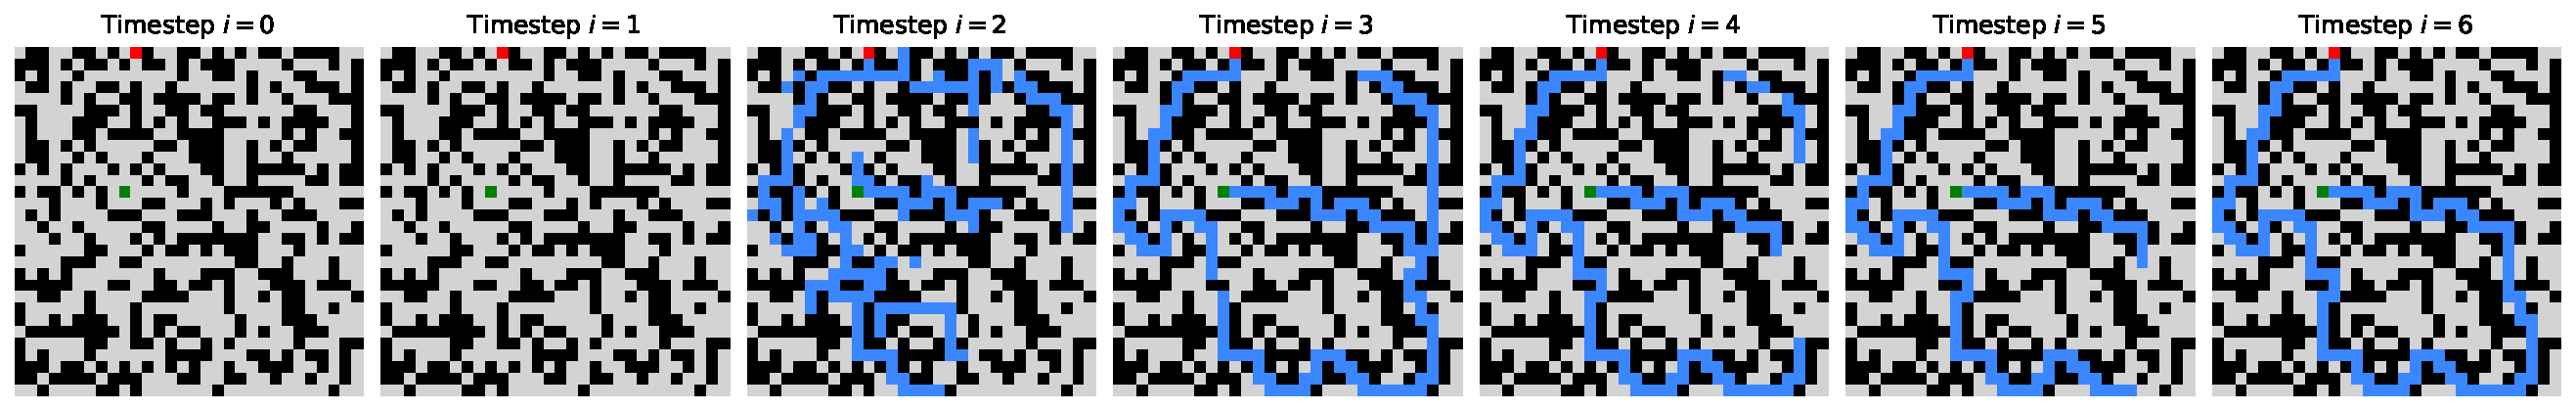
\includegraphics[width=1.1\linewidth]{figures/visualization/maze-100.pdf}%
  }\\
  % row
  \makebox[\linewidth][c]{%
    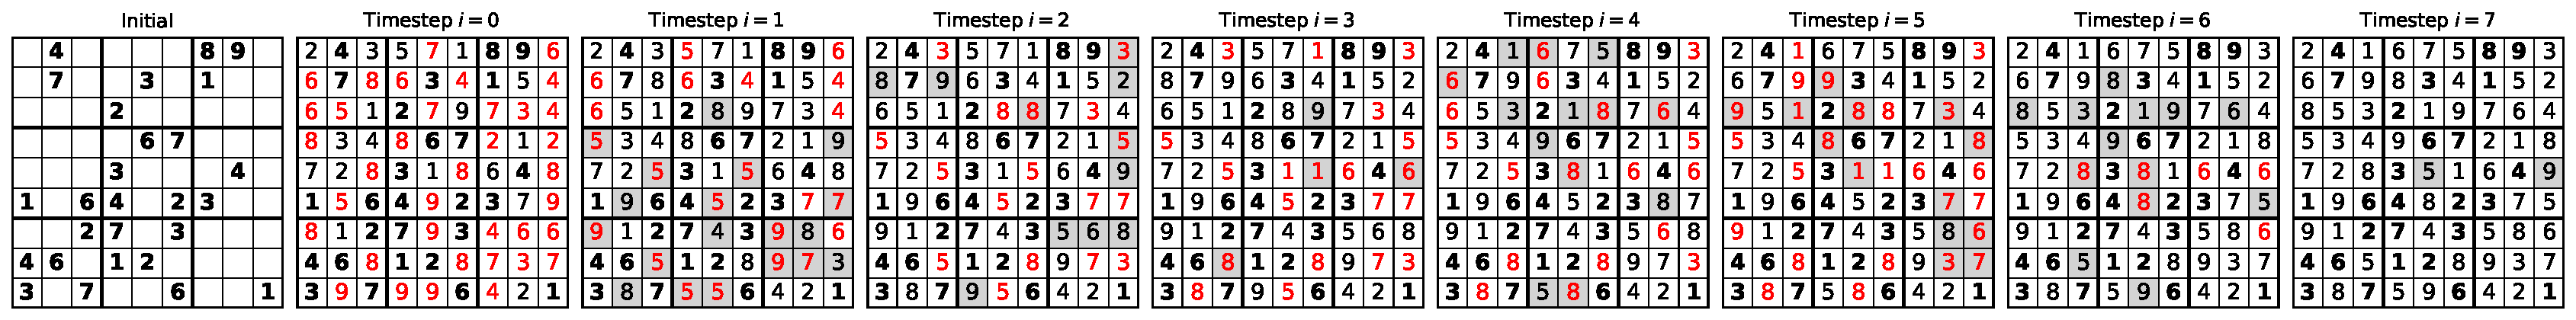
\includegraphics[width=1.1\linewidth]{figures/visualization/sudoku-hard-1.pdf}%
  }\\
    % row
  \makebox[\linewidth][c]{%
    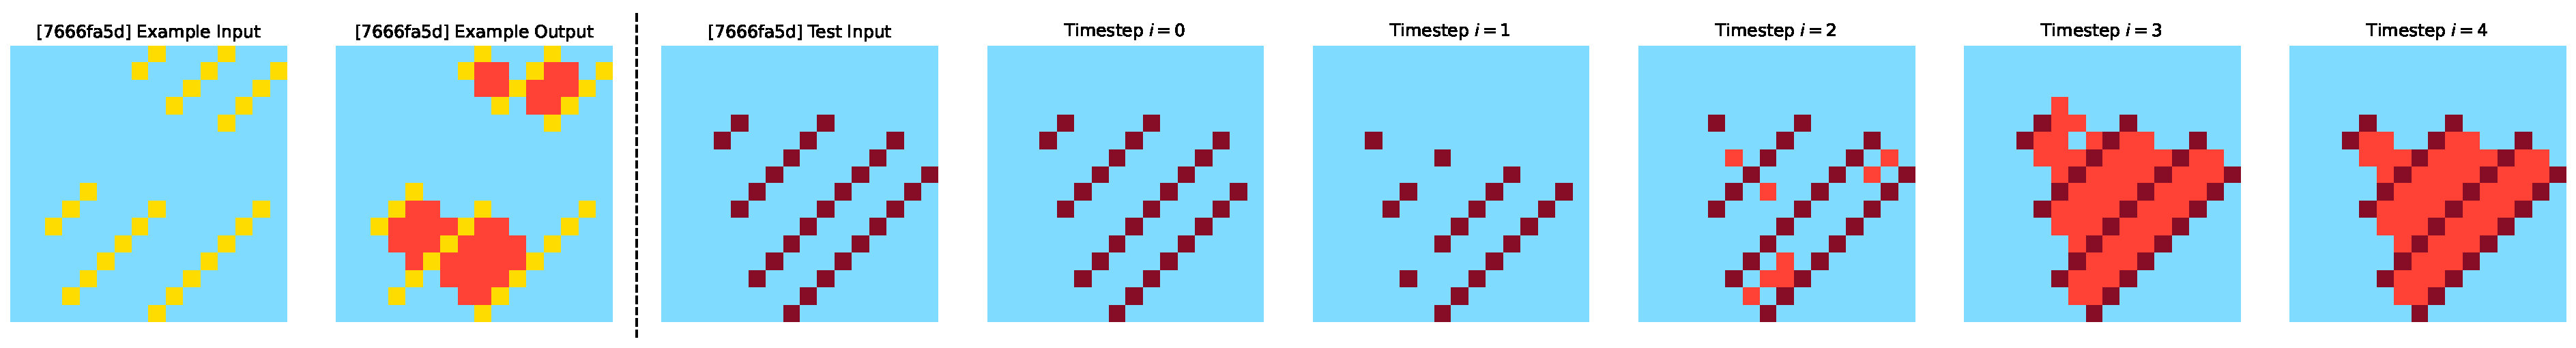
\includegraphics[width=1.1\linewidth]{figures/visualization/7666fa5d.pdf}%
  }\\
      % row
  \makebox[\linewidth][c]{%
    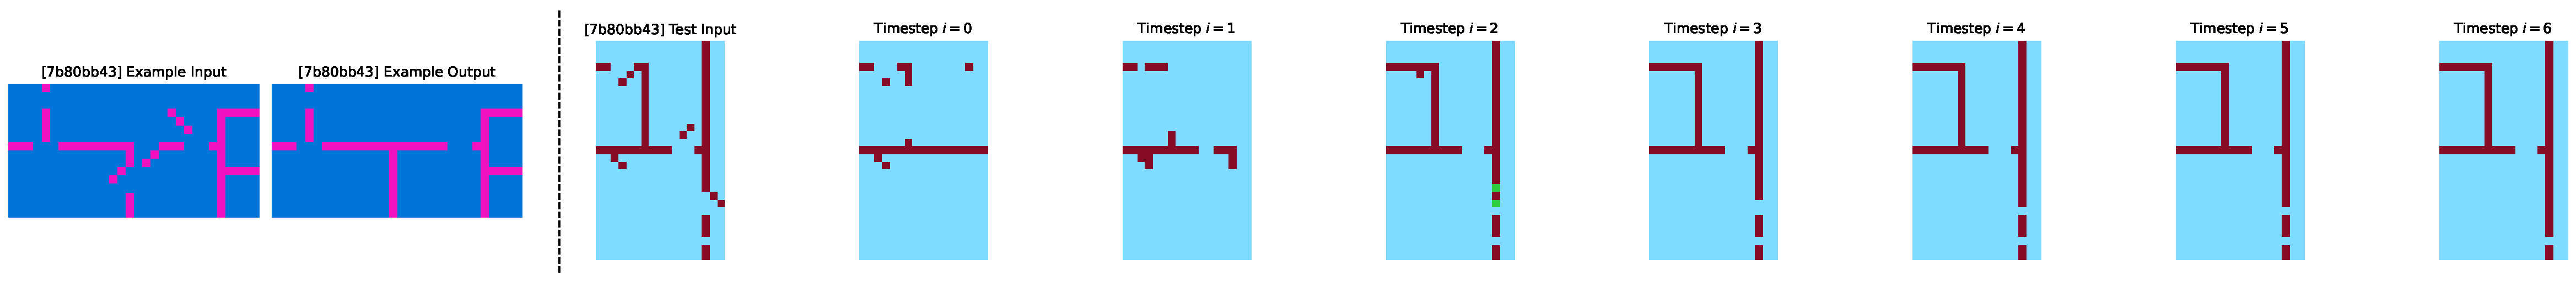
\includegraphics[width=1.1\linewidth]{figures/visualization/7b80bb43.pdf}%
  }
  \caption{\textbf{Visualization of intermediate predictions by HRM on benchmark tasks.} \textbf{Top:} \textit{Maze-Hard}—blue cells indicate the predicted path. \textbf{Middle:} \textit{Sudoku-Extreme}—bold cells represent initial givens; red highlights cells violating Sudoku constraints; grey shading indicates changes from the previous timestep.
  \textbf{Bottom:} ARC-AGI-2 Task—left: provided example input-output pair; right: intermediate steps solving the test input.}
  \label{fig:visualization}
\end{figure}

Although convergence is crucial for recurrent networks, standard RNNs are fundamentally limited by their tendency to converge too early. As the hidden state settles toward a fixed point, update magnitudes shrink, effectively stalling subsequent computation and capping the network’s effective depth. To preserve computational power, we actually want convergence to proceed very slowly--but engineering that gradual approach is difficult, since pushing convergence too far edges the system toward instability.

HRM is explicitly designed to counteract this premature convergence through a process we term \textit{hierarchical convergence}. During each cycle, the L-module (an RNN) exhibits stable convergence to a \textit{local equilibrium}. This equilibrium, however, depends on the high-level state $z_H$ supplied during that cycle. After completing the $T$ steps, the H-module incorporates the sub-computation's outcome (the final state $z_L$) and performs its own update. This $z_H$ update establishes a fresh context for the L-module, essentially ``restarting'' its computational path and initiating a new convergence phase toward a different local equilibrium.

This process allows the HRM to perform a sequence of distinct, stable, nested computations, where the H-module directs the overall problem-solving strategy and the L-module executes the intensive search or refinement required for each step. Although a standard RNN may approach convergence within $T$ iterations, the hierarchical convergence benefits from an enhanced effective depth of $NT$ steps. As empirically shown in \Cref{fig:forward-residual}, this mechanism allows HRM both to maintain high computational activity (forward residual) over many steps (in contrast to a standard RNN, whose activity rapidly decays) and to enjoy stable convergence. This translates into better performance at any computation depth, as illustrated in \Cref{fig:perf-layers}.

\paragraph{Approximate gradient}
Recurrent models typically use BPTT to compute gradients. However, BPTT requires storing the hidden states from the forward pass and then combining them with gradients during the backward pass, which demands $O(T)$ memory for T timesteps. This heavy memory burden forces smaller batch sizes and leads to poor GPU utilization, especially for large-scale networks. Additionally, because retaining the full history trace through time is biologically implausible, it is unlikely that the brain implements BPTT~\cite{LILLICRAP201982}. 

Fortunately, if a recurrent neural network converges to a fixed point, we can avoid unrolling its state sequence by applying backpropagation in a single step at that equilibrium point. Moreover, such a mechanism could plausibly be implemented in the brain using only local learning rules~\cite{Scellier2016EquilibriumPB, Eprop}. Based on this finding, we propose a one-step approximation of the HRM gradient--using the gradient of the last state of each module and treating other states as constant. The gradient path is, therefore, 
{\small\begin{quote}
    Output head → final state of the H-module → final state of the L-module → input embedding
\end{quote}}

The above method needs $O(1)$ memory, does not require unrolling through time, and can be easily implemented with an autograd framework such as PyTorch, as shown in \Cref{fig:pseudocode}. Given that each module only needs to back-propagate errors through its most recent local synaptic activity, this approach aligns well with the perspective that cortical credit assignment relies on short-range, temporally local mechanisms rather than on a global replay of activity patterns.

\begin{figure}[t]
  \centering
  %  row
  \makebox[\linewidth][c]{%
    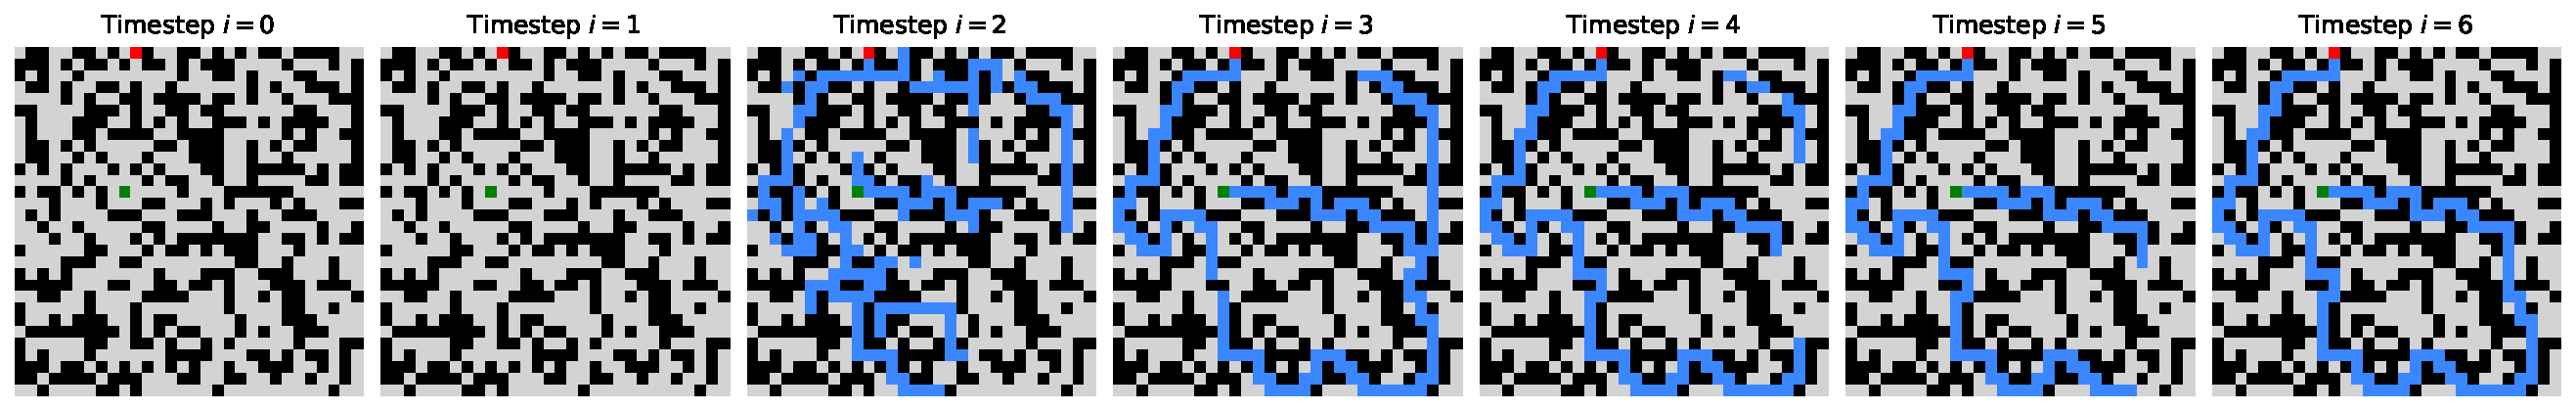
\includegraphics[width=1.1\linewidth]{figures/visualization/maze-100.pdf}%
  }\\
  % row
  \makebox[\linewidth][c]{%
    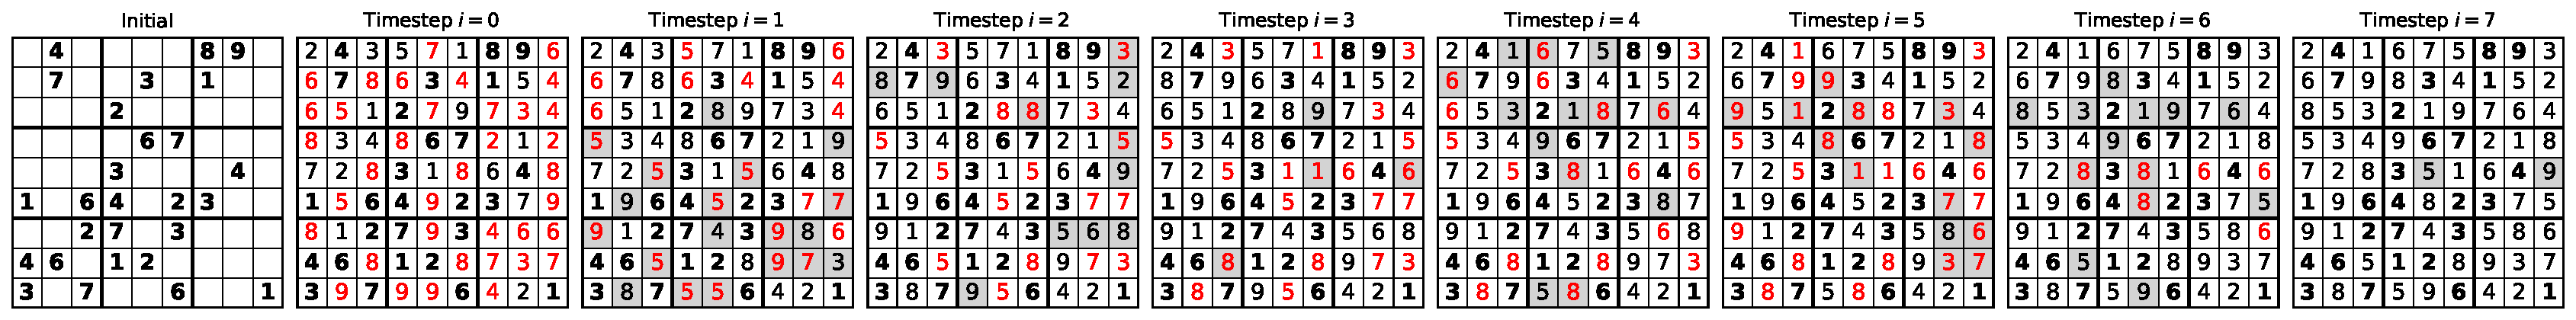
\includegraphics[width=1.1\linewidth]{figures/visualization/sudoku-hard-1.pdf}%
  }\\
    % row
  \makebox[\linewidth][c]{%
    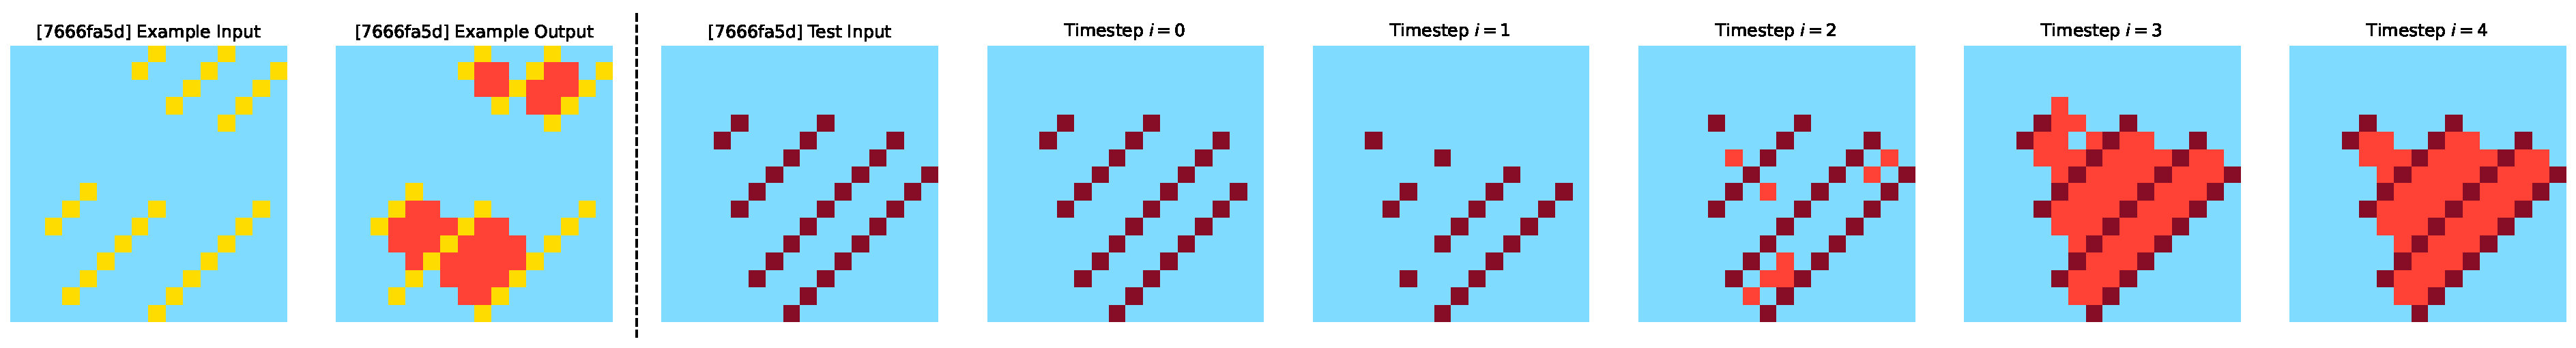
\includegraphics[width=1.1\linewidth]{figures/visualization/7666fa5d.pdf}%
  }\\
      % row
  \makebox[\linewidth][c]{%
    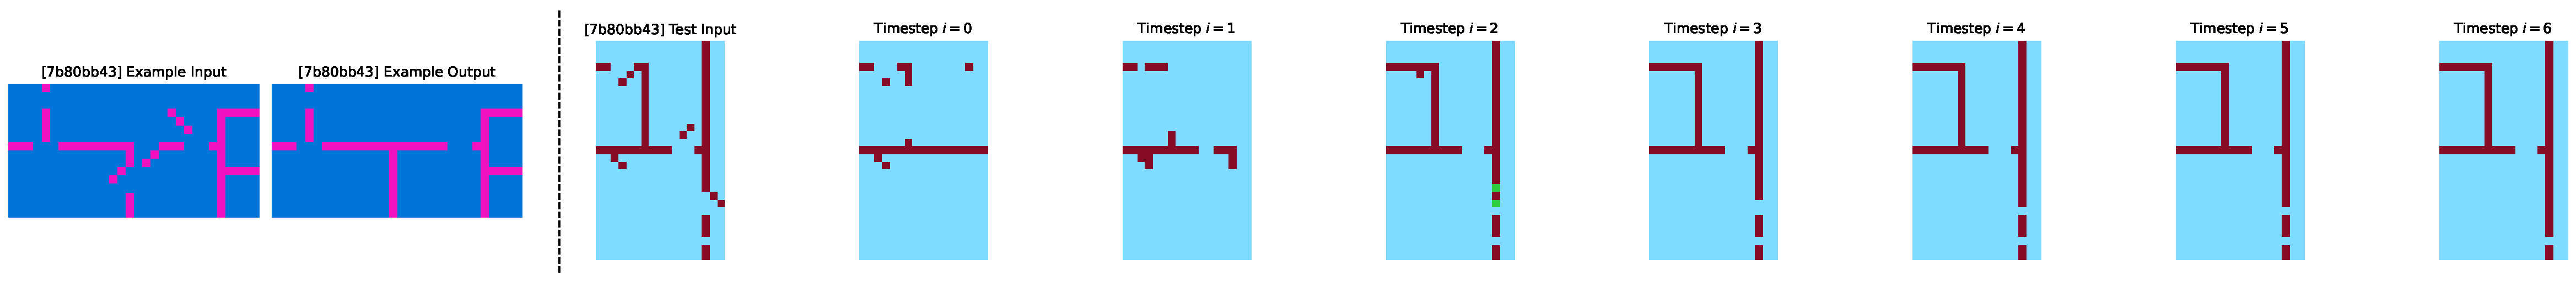
\includegraphics[width=1.1\linewidth]{figures/visualization/7b80bb43.pdf}%
  }
  \caption{\textbf{Visualization of intermediate predictions by HRM on benchmark tasks.} \textbf{Top:} \textit{Maze-Hard}—blue cells indicate the predicted path. \textbf{Middle:} \textit{Sudoku-Extreme}—bold cells represent initial givens; red highlights cells violating Sudoku constraints; grey shading indicates changes from the previous timestep.
  \textbf{Bottom:} ARC-AGI-2 Task—left: provided example input-output pair; right: intermediate steps solving the test input.}
  \label{fig:visualization}
\end{figure}

The one-step gradient approximation is theoretically grounded in the mathematics of Deep Equilibrium Models (DEQ)~\citep{bai2019deep} which employs the Implicit Function Theorem (IFT) to bypass BPTT, as detailed next. Consider an idealized HRM behavior where, during high-level cycle $k$, the L-module repeatedly updates until its state $z_L$ converges to a local fixed point $z_L^\star$. This fixed point, given the current high-level state $z_H^{k-1}$, can be expressed as
\begin{equation*}
    z_L^\star = f_L(z_L^\star, z_H^{k-1}, \tilde{x}; \theta_L) \;.
\end{equation*}
The H-module then performs a single update using this converged L-state:
\begin{equation*}
    z_H^k = f_H(z_H^{k-1}, z_L^\star; \theta_H) \;.
\end{equation*}
With a proper mapping $\mathcal{F}$, the updates to the high-level state can be written in a more compact form as $z_H^k = \mathcal{F}(z_H^{k-1}; \tilde{x}, \theta)$, where $\theta = (\theta_I, \theta_L)$, and the fixed-point can be written as $z_H^\star = \mathcal{F}(z_H^\star; \tilde{x}, \theta)$. Let $ J_{\mathcal{F}} = \frac{\partial \mathcal{F}}{\partial z_H}$ be the Jacobian of $\mathcal{F}$, and assume that the matrix $I - J_{\mathcal{F}}$ is invertible at $z_H^\star$ and that the mapping $\mathcal{F}$ is continuously differentiable. The Implicit Function Theorem then allows us to calculate the exact gradient of fixed point $z_H^\star$ with respect to the parameters $\theta$ without explicit backpropagation:
\begin{equation}
\label{eq:IFT-zH}
\frac{\partial z_H^\star}{\partial \theta} = \left( I - J_{\mathcal{F}} \big|_{z_H^\star} \right)^{-1} \frac{\partial \mathcal{F}}{\partial \theta} \bigg|_{z_H^\star} \;.
\end{equation}

Calculating the above gradient requires evaluating and inverting matrix $(I - J_{\mathcal{F}})$ that can be computationally expensive. Given the Neumann series expansion,
\begin{equation*}
(I - J_{\mathcal{F}})^{-1} = I + J_{\mathcal{F}} + J_{\mathcal{F}}^2 + J_{\mathcal{F}}^3 + \dots \,,
\end{equation*}
the so-called \textit{1-step gradient}~\cite{Geng2021OnTI} approximates the series by considering only its first term, i.e. $(I - J_{\mathcal{F}})^{-1} \approx I$, and leads to the following approximation of \Cref{eq:IFT-zH}:  
\begin{equation}
\label{eq:1-step-1}
\frac{\partial z_H^*}{\partial\theta_H} \approx \frac{\partial f_H}{\partial \theta_H},
\quad
\frac{\partial z_H^*}{\partial\theta_L}\approx \frac{\partial f_H}{\partial z^*_L} \cdot \frac{\partial z^*_L}{\partial \theta_L},
\quad
\frac{\partial z_H^*}{\partial\theta_I} \approx \frac{\partial f_H}{\partial z^*_L} \cdot
\frac{\partial z^*_L}{\partial \theta_I} \;.
\end{equation}
% \todoy{Replaced $\tilde{x}$ with $\theta_I$}
The gradients of the low-level fixed point, $\frac{\partial z^*_L}{\partial \theta_L}$ and $\frac{\partial z^*_L}{\partial \theta_I}$, can also be approximated using another application of the 1-step gradient:
\begin{equation}
\label{eq:1-step-2}
\frac{\partial z^*_L}{\partial \theta_L} \approx \frac{\partial f_L}{\partial \theta_L},
\quad
\frac{\partial z^*_L}{\partial \theta_I} \approx \frac{\partial f_L}{\partial \theta_I} \;.
\end{equation}
By substituting \Cref{eq:1-step-2} back into \Cref{eq:1-step-1}, we arrive at the final simplified gradients.

Before defining our loss function, we must first introduce two key elements of our proposed method: \textit{deep supervision} and \textit{adaptive computational time}.

\paragraph{Deep supervision}
Inspired by the principle that periodic neural oscillations regulate when learning occurs in the brain~\cite{BEGUS2020100810}, we incorporate a deep supervision mechanism into HRM, as detailed next. 

Given a data sample $(x, y)$, we run multiple forward passes of the HRM model, each of which we refer to as a \textit{segment}. Let $M$ denote the total number of segments executed before termination. For each segment $m \in \{1, \dots, M\}$, let $z^m = (z^{mNT}_H, z^{mNT}_L)$ represent the hidden state at the conclusion of segment $m$, encompassing both high-level and low-level state components.

At each segment $m$, we apply a deep supervision step as follows:
\begin{enumerate}
\vspace{-0.15in}
    \item Given the state $z^{m-1}$ from the previous segment, compute the next state $z^m$ and its associated output $\hat{y}^m$ through a forward pass in the HRM model:
    \begin{equation*}
    (z^m, \hat{y}^m) \leftarrow \textsc{HRM}(z^{m-1}, x; \theta)
    \end{equation*}
    \item Compute the loss for the current segment:
    \begin{equation*}
    L^m \leftarrow \textsc{Loss}(\hat{y}^m, y)
    \end{equation*}
    \item Update parameters:
    \begin{equation*}
    \theta \leftarrow \textsc{OptimizerStep}(\theta, \nabla_{\theta} L^m)
    \end{equation*}
\end{enumerate}
The crucial aspect of this procedure is that the hidden state $z^m$ is ``detached'' from the computation graph before being used as the input state for the next segment. Consequently, gradients from segment $m+1$ do not propagate back through segment $m$, effectively creating a 1-step approximation of the gradient of the recursive deep supervision process~\citep{DEQ-Flow, Ramzi2021SHINEST}. This approach provides more frequent feedback to the H-module and serves as a regularization mechanism, demonstrating superior empirical performance and enhanced stability in deep equilibrium models when compared to more complex, Jacobian-based regularization techniques~\citep{DEQ-Flow, Bai2021StabilizingEM}. \Cref{fig:pseudocode} shows pseudocode of deep supervision training.

\paragraph{Adaptive computational time (ACT)}
The brain dynamically alternates between automatic thinking (``System 1'') and deliberate reasoning (``System 2'')~\citep{kahneman2011thinking}. Neuroscientific evidence shows that these cognitive modes share overlapping neural circuits, particularly within regions such as the prefrontal cortex and the default mode network~\citep{lieberman2007social,buckner2008brain}. This indicates that the brain dynamically modulates the ``runtime'' of these circuits according to task complexity and potential rewards~\citep{raichle2015brain,westbrook2015cognitive}.

Inspired by the above mechanism, we incorporate an adaptive halting strategy into HRM that enables ``thinking, fast and slow''. This integration leverages deep supervision and uses the Q-learning algorithm~\cite{Sutton-Barto-2018} to adaptively determine the number of segments. A Q-head uses the final state of the H-module to predict the Q-values $\hat{Q}^m = (\hat{Q}^m_\text{halt}, \hat{Q}^m_\text{continue})$ of the ``halt'' and ``continue'' actions:
\begin{equation*}
    \hat{Q}^m = \sigma(\theta_Q^\top z_H^{mNT})\,,
\end{equation*}
where $\sigma$ denotes the sigmoid function applied element-wise. The halt or continue action is chosen using a randomized strategy as detailed next. Let $M_{\max}$ denote the maximum number of segments (a fixed hyperparameter) and $M_{\min}$ denote the minimum number of segments (a random variable). The value of $M_{\min}$ is determined stochastically: with probability $\varepsilon$, it is sampled uniformly from the set $\{2,\cdots,M_{\max}\}$ (to encourage longer thinking), and with probability $1-\varepsilon$, it is set to 1. The halt action is selected under two conditions: when the segment count surpasses the maximum threshold $M_{\max}$, or when the estimated halt value $\hat{Q}_\text{halt}$ exceeds the estimated continue value $\hat{Q}_\text{continue}$ and the segment count has reached at least the minimum threshold $M_{\min}$.

The Q-head is updated through a Q-learning algorithm, which is defined on the following episodic Markov Decision Process (MDP). The state of the MDP at segment $m$ is $z^m$, and the action space is $\{\text{halt}, \text{continue}\}$. Choosing the action ``halt'' terminates the episode and returns a binary reward indicating prediction correctness, i.e., $\mathbf{1}\{\hat{y}^m = y\}$. Choosing ``continue'' yields a reward of 0 and the state transitions to $z^{m+1}$. Thus, the Q-learning targets for the two actions $\hat{G}^m = (\hat{G}^m_\text{halt}, \hat{G}^m_\text{continue})$ are given by
\begin{align*}
\hat{G}_\text{halt}^m &= \mathbf{1}\{\hat{y}^m = y\}\,, \\
\hat{G}_\text{continue}^m &= 
\begin{cases}
\hat{Q}_\text{halt}^{m+1}, & \text{if $m \geq N_{\max}$}\,,\\[6pt]
\max(\hat{Q}_\text{halt}^{m+1}, \hat{Q}_\text{continue}^{m+1})\,, & \text{otherwise}\;.
\end{cases}
\end{align*}
We can now define the loss function of our learning procedure. The overall loss for each supervision segment combines both the Q-head loss and the sequence-to-sequence loss:
\begin{equation*}
    L^m_\text{ACT} = \textsc{Loss}(\hat{y}^m, y) + \textsc{BinaryCrossEntropy}(\hat{Q}^m, \hat{G}^m) \;.
\end{equation*}
Minimizing the above loss enables both accurate predictions and nearly optimal stopping decisions. 

Selecting the ``halt'' action ends the supervision loop. In practice, sequences are processed in batches, which can be easily handled by substituting any halted sample in the batch with a fresh sample from the dataloader.

\Cref{fig:act} presents a performance comparison between two HRM variants: one incorporating ACT and another employing a fixed computational step count equivalent to ACT's $M_{\max}$ parameter. It shows that ACT effectively adapts its computational resources based on task complexity, achieving significant computational savings with minimal impact on performance.

\begin{figure}[t!]
\centering
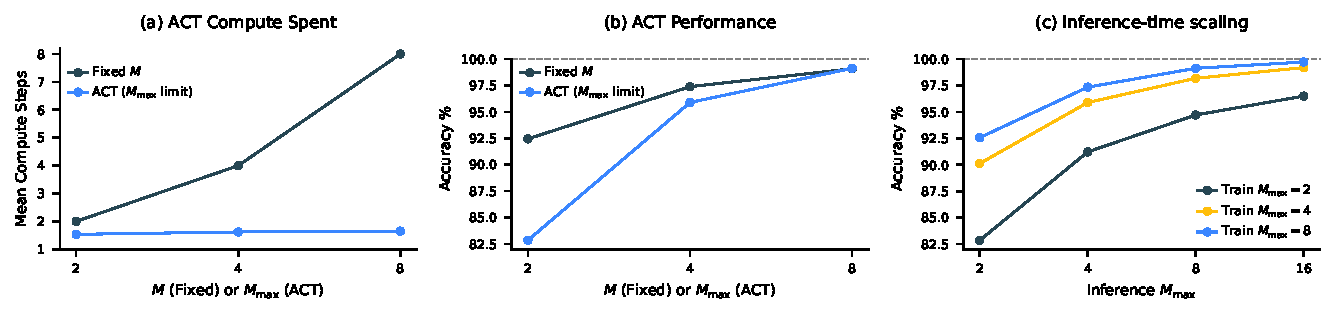
\includegraphics[width=\linewidth]{figures/act/act.pdf} 
\caption{\textbf{Effectiveness of Adaptive Computation Time (ACT)} on the \textit{Sudoku-Extreme-Full}.
\textbf{(a)} Mean compute steps used by models with ACT versus models with a fixed number of compute steps ($M$). ACT maintains a low and stable number of average compute steps even as the maximum limit ($M_{\max}$) increases.
\textbf{(b)} Accuracy comparison. The ACT model achieves performance comparable to the fixed-compute model while utilizing substantially fewer computational steps on average.
\textbf{(c)} Inference-time scalability. Models trained with a specific $M_{\max}$ can generalize to higher computational limits during inference, leading to improved accuracy. For example, a model trained with $M_{\max}=8$ continues to see accuracy gains when run with $M_{\max}=16$ during inference.}
\label{fig:act}
\end{figure}

\paragraph{Inference-time scaling}
An effective neural model should exploit additional computational resources during inference to enhance performance. As illustrated in \Cref{fig:act}-(c), HRM seamlessly achieves inference-time scaling by simply increasing the computational limit parameter, $M_{\max}$ without requiring further training or architectural modifications.

Additional compute is especially effective for tasks that demand deeper reasoning. On Sudoku---a problem that often requires long-term planning---HRM exhibits strong inference-time scaling. On the other hand, we find that extra computational resources yield minimal gains in ARC-AGI challenge, as solutions generally require only a few transformations.

\paragraph{Stability of Q-learning in ACT}
The deep Q-learning that underpins our ACT mechanism is known to be prone to instability, often requiring stabilization techniques such as replay buffers and target networks~\citep{DQN}, which are absent in our design. Our approach, however, achieves stability through the intrinsic properties of our model and training procedure. Recent theoretical work by \citet{PQN2025} shows that Q-learning can achieve convergence if network parameters are bounded, weight decay is incorporated during training, and post-normalization layers are implemented.
Our model satisfies these conditions through its Post-Norm architecture that employs RMSNorm (a layer normalization variant) and the AdamW optimizer. AdamW has been shown to solve an $L_\infty$-constrained optimization problem, ensuring that model parameters remain bounded by $1/\lambda$ \citep{Xie2024ImplicitBO}.

\paragraph{Architectural details}
We employ a sequence-to-sequence architecture for HRM. Both input and output are represented as token sequences: $x = (x_1,\ldots,x_l)$ and $y = (y_1,\ldots,y_{l^\prime})$ respectively. The model includes an embedding layer $f_I$ that converts discrete tokens into vector representations, and an output head $f_O(z; \theta_O) = \text{softmax}(\theta_O z)$ that transforms hidden states into token probability distributions $\hat{y}$. For small-sample experiments, we replace softmax with stablemax~\cite{PBMB-2025} to improve generalization performance. The sequence-to-sequence loss is averaged over all tokens, $\textsc{Loss}(\hat{y}, y) = \frac{1}{l^\prime} \sum_{i=1}^{l^\prime}\log p(y_i)$, where $p(y_i)$ is the probability that distribution $\hat{y}_i$ assigns to token $y_i$. The initial hidden states $z^0$ are initialized by sampling from a truncated normal distribution with standard deviation of 1, truncation of 2, and kept fixed throughout training.

Both the low-level and high-level recurrent modules $f_L$ and $f_H$ are implemented using encoder-only Transformer~\cite{vaswani2017attention} blocks with identical architectures and dimensions. 
These modules take multiple inputs, and we use straightforward element-wise addition to combine them, though more sophisticated merging techniques such as gating mechanisms could potentially improve performance and is left for future work. For all Transformer blocks in this work---including those in the baseline models---we incorporate the enhancements found in modern LLMs (based on Llama~\cite{meta2024llama3} architectures). These improvements include Rotary Positional Encoding~\citep{SHLPBL-2024}, Gated Linear Units~\cite{Shazeer2020GLUVI}, RMSNorm~\cite{Zhang2019RootMS}, and the removal of bias terms from linear layers. 

Furthermore, both HRM and recurrent Transformer models implement a Post-Norm architecture with weights initialized via truncated LeCun Normal initialization~\cite{Klambauer2017SelfNormalizingNN, jax_lecun_normal_initializer,lecun2002efficient}, while the scale and bias parameters are excluded from RMSNorm. All parameters are optimized using the Adam-atan2 optimizer~\citep{EXWANLGSKLP-2024}, a scale-invariant variant of Adam~\citep{KB-2017}, combined with a constant learning rate that includes linear warm-up.